\documentclass[11pt]{article}

\usepackage[margin=1in]{geometry}
\usepackage{amsmath,amssymb,amsthm}
\usepackage{graphicx}
\usepackage[hidelinks]{hyperref}

\newtheorem{theorem}{Theorem}

\newcommand{\NPSS}{Naor--Peres--Schramm--Sheffield}

\begin{document}

\begin{center}
{\Large Literature status: planar and doubling metrics have Markov type \(2\)}

\medskip
{\small Run \texttt{fa\_banach\_001}; source arXiv:math/0410422}
\end{center}

\section*{Source question}

\NPSS{} introduced and studied Markov type methods for smooth Banach spaces,
trees, hyperbolic spaces, and several metric families.  In the discussion
section they ask, in belief form, whether planar graphs and doubling spaces
have Markov type \(2\).  The same item also mentions CAT(0) spaces; this
packet does not address that adjacent part.

\begin{figure}[h]
\centering

\includegraphics[width=\textwidth]{figures/open_problem_crop.png}
\caption{arXiv:math/0410422, page 22, item 7 in the discussion section.}
\end{figure}

The target status question recorded here is:
\[
  \text{Do planar graph metrics and doubling metric spaces have Markov type }2?
\]

\section*{Supporting literature status}

Ding--Lee--Peres later introduced threshold embeddings as a tool for
controlling Markov type.  Their abstract states that if a metric space
threshold-embeds into Hilbert space, then it has Markov type \(2\), and then
draws the explicit consequence for planar graph metrics and doubling metrics.
The abstract also says that this answers questions of \NPSS{}.

\begin{figure}[h]
\centering
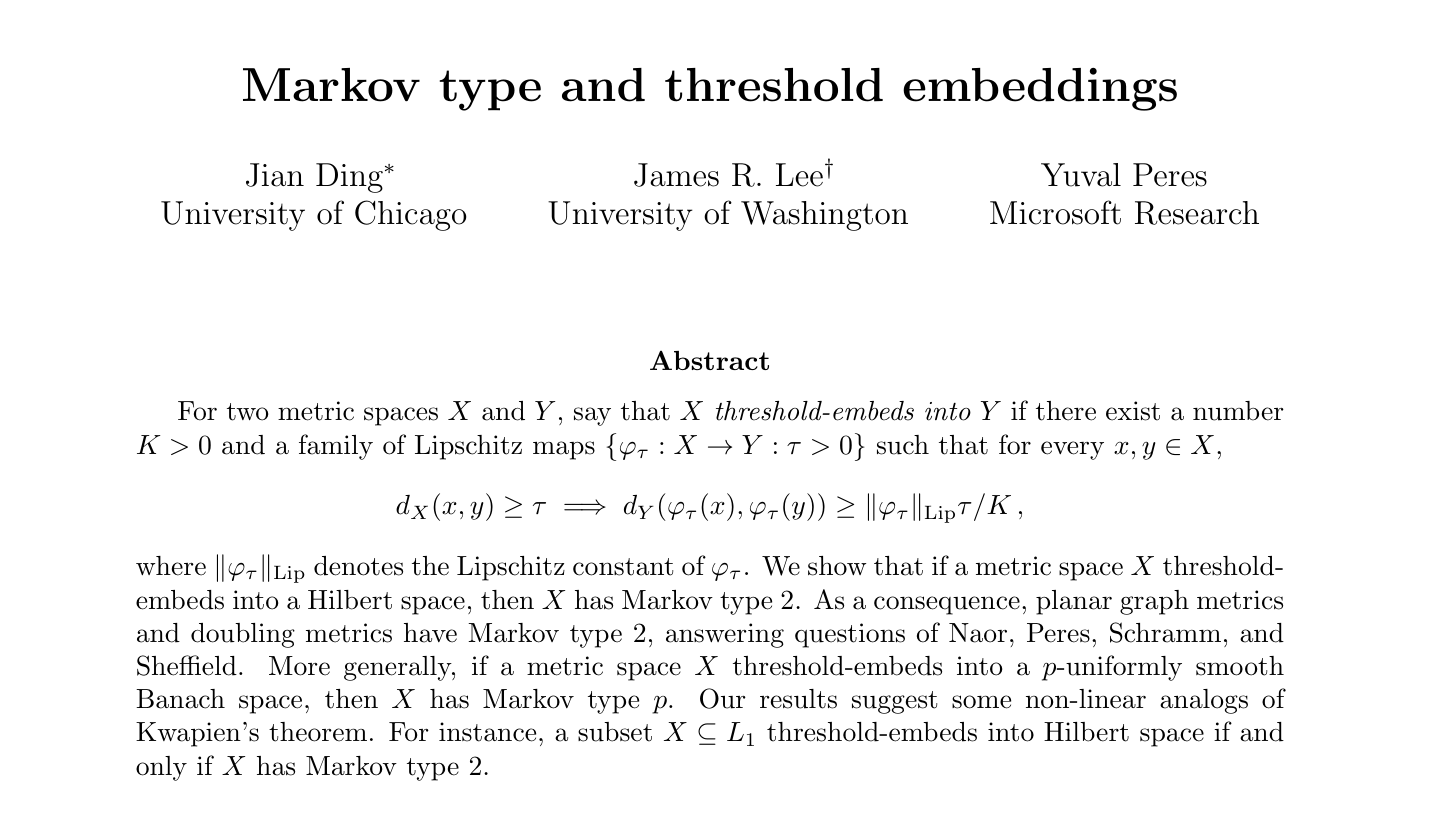
\includegraphics[width=\textwidth]{figures/supporting_answer_crop.png}
\caption{arXiv:1208.6088, page 1: the abstract states the planar and doubling
Markov type \(2\) conclusion and identifies it as answering \NPSS{}.}
\end{figure}

The introduction of the supporting paper further identifies the exact NPSS
beliefs: it says that \NPSS{} had stated that planar graph metrics and doubling
metrics should have Markov type \(2\), while only Markov type \(2-\varepsilon\)
was known there, and then says the paper resolves these questions.

\section*{Idea of the proof identification}

This packet is not an original proof.  The identification is direct: the source
paper asks for Markov type \(2\) of planar graph metrics and doubling spaces,
and the supporting paper explicitly proves those two assertions and says they
answer questions of \NPSS{}.

At a high level, the supporting proof works by relaxing bi-Lipschitz embeddings
to threshold embeddings.  Ding--Lee--Peres prove that threshold embedding into
Hilbert space is enough to force Markov type \(2\).  They then use known
random-partition and threshold-embedding results for planar metrics and
doubling metrics to obtain the desired Markov type \(2\) conclusion.

\begin{theorem}[Literature answer]
Planar graph metrics and doubling metric spaces have Markov type \(2\).
\end{theorem}

\begin{proof}
This is the explicit consequence stated in the abstract of Ding--Lee--Peres
\cite{DingLeePeresThreshold}.  The same paper's introduction identifies the
claim as resolving the corresponding questions from \NPSS{}
\cite{NaorPeresSchrammSheffieldMarkov}.  Hence the planar and doubling parts
of the source discussion item are answered affirmatively in later literature.
\end{proof}

\section*{Verification notes and limitations}

The source paper and supporting paper are distinct.  The supporting paper
explicitly names \NPSS{} when saying that planar graph metrics and doubling
metrics have Markov type \(2\), and its introduction identifies the same
questions from the source paper.

This packet does not claim any status for the CAT(0) part of the source item.
It also does not address the other discussion questions in arXiv:math/0410422,
including the nonlinear Maurey constant, the \(L_1\)-valued extension question,
the best tree constant, or maximal Markov type.

Bounded duplicate/status check: I searched the run's cheap indexes for
arXiv id \texttt{0410422}, the source title, Markov type, planar graphs,
doubling spaces, and nearby title keywords, finding no prior packet or
attempt for this exact target.  I searched local parsed sources and references
for \texttt{1208.6088}, ``Markov type and threshold embeddings'', and
``Ding Lee Peres'', locating the supporting paper and publication data.  A web
search over the exact supporting-paper title and target phrases found the same
answer source and no conflicting status for the planar/doubling result.

This packet is a literature-status record only.  It should not be counted as a
new proof, partial result, or counterexample produced by this run.

\begin{thebibliography}{9}

\bibitem{NaorPeresSchrammSheffieldMarkov}
A. Naor, Y. Peres, O. Schramm, and S. Sheffield,
\emph{Markov chains in smooth Banach spaces and Gromov hyperbolic metric
spaces},
arXiv:math/0410422, 2004.

\bibitem{DingLeePeresThreshold}
J. Ding, J. R. Lee, and Y. Peres,
\emph{Markov type and threshold embeddings},
Geom. Funct. Anal. 23(4), 1207--1229, 2013;
arXiv:1208.6088.

\end{thebibliography}

\end{document}
